\documentclass[aip,jcp,reprint,a4paper,onecolumn,amsmath]{revtex4-1}
% Options for onecolumn and a4paper
\linespread{1.0}
\usepackage[expansion,protrusion,tracking=smallcaps]{microtype}
\usepackage{listings,tikz,tikz-3dplot,xcolor,upquote}
\tikzset{
  dot/.style = {draw,fill,circle,inner sep=1pt}
}
\lstset{
  basicstyle = \small\ttfamily,
  keywordstyle = \color{blue!80!black},
  commentstyle = \color{green!40!black},
  columns = fullflexible,
  xleftmargin = 1em
}
\lstnewenvironment{espresso}[1][]%
  {\lstset{language=python,#1}}%
  {}
\lstnewenvironment{bash}[1][]%
  {\lstset{keywordstyle = \color{red!80!blue},keywords={\$},#1}}%
  {}
\usepackage{xspace}
\newcommand\code{\lstinline}
\newcommand{\es}{\mbox{\textsf{ESPResSo}}\xspace}
\newcommand\codees{\lstinline[language=python]}
\begin{document}
\title{Active Matter Tutorial}
\author{Joost de Graaf}
\email[]{\texttt{jgraaf@icp.uni-stuttgart.de}}
\author{Henri Menke}
\email[]{\texttt{henri@icp.uni-stuttgart.de}}
\affiliation{Institute for Computational Physics,
  Universit\"at Stuttgart,
  Allmandring 3,
  D-70569 Stuttgart,
  Germany}

\begin{abstract}
In this tutorial we explore the ways to simulate self-propulsion in the simulation software package \es{}. We consider three examples that illustrate the properties of these systems. First, we study the concept of enhanced diffusion of a self-propelled particle. Second, we investigate rectification in an asymmetric geometry. Finally, we determine the flow field around a self-propelled particle using lattice-Boltzmann simulations (LB). These three subsections should give insight into the basics of simulating active matter with \es{}. This tutorial assumes basic knowledge of Python and \es{}, as well as the use of lattice-Boltzmann within \es{}. It is therefore recommended to go through the relevant tutorials first, before attempting this one.
\end{abstract}

\maketitle

\section{\label{sec:active}Active Particles}

Active matter is a term that describes a class of systems, in which energy is constantly consumed to perform work. These systems are therefore highly out-of-equilibrium (thermodynamically) and (can) thus defy description using the standard framework of statistical mechanics. Active systems are, however, ubiquitous. On our length scale, we encounter flocks of birds~\cite{Ballerini_08}, schools of fish~\cite{Katz_11}, and, of course, humans~\cite{Helbing_00,Zhang_13,Sliverberg_13}; on the mesoscopic level examples are found in bacteria~\cite{Sokolov_07,Schwarz-Linek_12,Reufer_14}, sperm~\cite{Woolley_03,Riedel_05,Ma_14}, and algae~\cite{Polin_09,Geyer_13}; and on the nanoscopic level, transport along the cytoskeleton is achieved by myosin motors~\cite{Mizuno07}. This exemplifies that range of length scales which the field of active matter encompasses, as well as its diversity. Recent years have seen a huge increase in studies into systems consisting of self-propelled particles, in particular artificial ones in the colloidal regime~\cite{ismagilov,Paxton_04,Wang_06,Brown,Ebbens,Ebbens_12,Howse_07,Valadares_10,simmchen,Yoshinaga,Baraban_13a,Buttinoni_12,Solovev_09,Mei_11}. These self-propelled colloids show promise as physical model systems for complex biological behavior (bacteria moving collectively) and could be used to answer fundamental questions concerning out-of-equilibrium statistical physics~\cite{Cates_12,Cates_14}. Simulations can also play an important role in this regard, as the parameters are more easily tunable and the results `cleaner' than in experiments. The above should give you some idea of the importance of the field of active matter and why you should be interested in performing simulations in it.

\section{\label{sec:swimming}Active Particles in ESPResSo}

The current development master of \es{} ships with the new \code{ENGINE} feature. N.B. There is currently no release version supporting this feature. \code{ENGINE} offers intuitive syntax for adding self-propulsion to a particle. The propulsion will occur along the vector that defines the orientation of the particle (henceforth referred to as `director'). In \es{} the orientation of the particle is defined by a quaternion; this in turn defines a rotation matrix that acts on the particle's initial orientation (along the z-axis), which then defines the particles current orientation through the matrix-oriented vector~\cite{UG,Limbach_06,Arnold_13}. Within the \code{ENGINE} feature there are two ways of setting up a self-propelled particle, with and without hydrodynamic interactions. The particle without hydrodynamic interactions will be discussed first, as it is the simplest case.

\subsection{\label{sub:langevin}Self-Propulsion without Hydrodynamics}

For this type of self-propulsion the Langevin thermostat is exploited. The Langevin thermostat causes a particle to experience a velocity-dependent friction~\cite{UG}. When a constant force is applied along the director, the friction causes the particle to attain a terminal velocity, due to the balance of driving and friction force, see Fig.~\ref{fig:balance}. The exponent with which the particle's velocity relaxes towards this value, depends on the strength of the friction and the mass of the particle. The \code{ENGINE} feature implies that rotation of the particles (the \code{ROTATION} feature) is compiled into \es{}. The particle can thus reorient due to external torques or due to thermal fluctuations, whenever the rotational degrees of freedom are thermalized. This `engine' building block can be connected to other particles,~\textit{e.g.}, via the virtual sites (rigid bonds)~\cite{UG} to construct complex self-propelled objects.

\begin{figure}[!htb]
\begin{center}
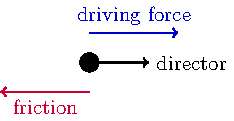
\includegraphics[scale=1.0]{FIGURES/friction}
\end{center}
\caption{\label{fig:balance}A balance of the driving force in the direction defined by the `director' unit vector and the friction due to the Langevin thermostat results in a constant terminal velocity.}
\end{figure}

The syntax for the Langevin-based swimming is incorporated in the \codees{ParticleHandle} command of \es{}. You can either set up the self-propulsion during the creation of a particle or at a later stage. In the following example we set up a particle with ID 0 at the position $(1,1,1)$ and set its terminal velocity to $1.0$.
\begin{espresso}
system.part.add(pos=[1,1,1],swimming={'v_swim':1.0})
\end{espresso}
As you can see, the keyword for setting up the engine is \codees{swimming}. The code \codees{'v_swim':1.0} sets the terminal velocity to $1.0$ (in MD units). Setting the terminal velocity directly is possible, since the terminal velocity is simply the ratio of the applied driving force and Langevin friction coefficient. It is also possible to set the driving force directly, which requires you to calculate/compute the terminal velocity. This can be achieved by replacing \codees{v_swim} with \codees{f_swim}. Please note, that the options \codees{v_swim} and \codees{f_swim} are mutually exclusive. Also, one is limited to the force/velocity and time step that can be used, by the stability criteria on the Langevin algorithm itself.

To modify a passive particle (switch on self-propulsion) or deactivate activity, one can use the following commands. Suppose a passive particle with, say ID 1, has been set up, we can add self-propulsion to it by specifying
\begin{espresso}
system.part[1].swimming = {'f_swim':0.03}
\end{espresso}
Finally, a particle's activity can be switched off, by setting either \codees{v_swim} or \codees{f_swim} to zero
\begin{espresso}
system.part[0].swimming = {'f_swim':0.0}
\end{espresso}
on the particle with ID 0 in this case. The numerical values of \codees{v_swim} and \codees{f_swim} in these examples are completely arbitrary and crucially depend on all other parameters of your simulation, such as friction, temperature, interactions, etc. Please consult the User Guide~\cite{UG} for additional information.

\subsection{\label{sub:lattice}Self-Propulsion with Hydrodynamics}

In situations where hydrodynamic interactions between swimmers or swimmers and objects are of importance, we use the lattice-Boltzmann (LB) to propagate the fluid's momentum diffusion. This requires the additional activation of the \code{LB} or \code{LB_GPU} feature in \es{}~\cite{UG,Arnold_13,roehm12}. We recommend the GPU-based variant of LB in \es{}, since it is much faster. Moreover, the current implementation of the CPU self-propulsion is limited to one CPU. This is because the ghost-node structure of the \es{} cell-list code does not allow for straightforward MPI parallellization of the swimmer objects across several CPUs.

Of particular importance for self-propulsion at low Reynolds number is the fact that active systems (bacteria, sperm, algae, but also artificial chemically powered swimmers) are force free. That is, the flow field around one of these objects does not contain a monopolar (Stokeslet) contribution. In the case of a sperm cell, see Fig.~\ref{fig:pusher-puller}(a), the reasoning is as follows. The whip-like tail pushes against the fluid and the fluid pushes against the tail, at the same time the head experiences drag, pushing against the fluid and being pushed back against by the fluid. This ensures that both the swimmer and the fluid experience no net force. However, due to the asymmetry of the distribution of forces around the swimmer, the fluid flow still causes net motion. When there is no net force on the fluid, the lowest-order multipole that can be present is a hydrodynamic dipole. Since a dipole has an orientation, there are two types of swimmer: pushers and pullers. The distinction is made by whether the particle pulls fluid in from the front and back, and pushes it out towards its side (puller), or vice versa (pusher), see Fig.~\ref{fig:pusher-puller}(c,d).

\begin{figure}[!htb]
\begin{center}
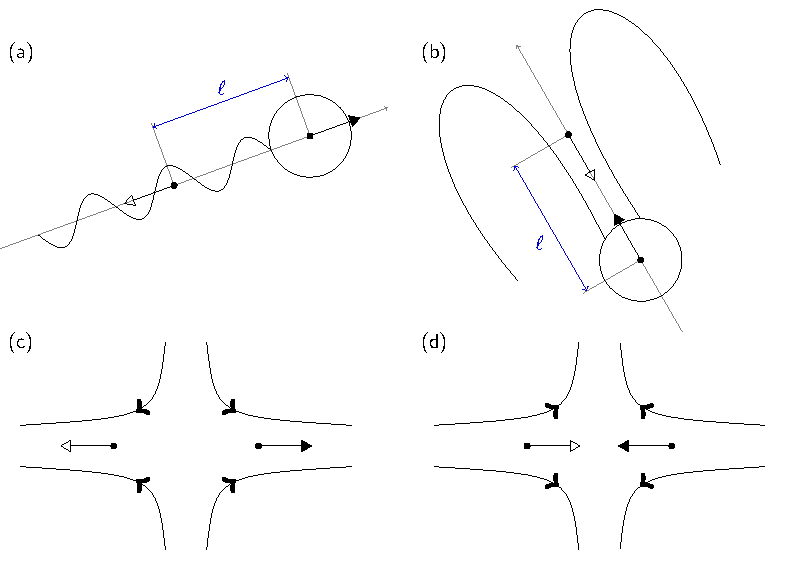
\includegraphics[scale=1.0]{FIGURES/pusher-puller}
\end{center}
\caption{\label{fig:pusher-puller}(a) Illustration of a sperm cell modeled using our two-point swimmer code. The head is represented by a solid particle, on which a force is acting (black arrow). In the fluid a counter force is applied (white arrow). This generates a pusher-type particle. (b) Illustration of the puller-type Chlamydomonas algae, also represented by our two-point swimmer. (c,d) Sketch of the flow-lines around the swimmers: (c) pusher and (d) puller.}
\end{figure}

In \es{} one can model both pushers and pullers using the following command. Say we want to set up a pusher with ID 0 at the position $(1,1,1)$ that has a dipolar strength of 0.1. Then we need to first set up the LB fluid (on the GPU) by invoking
\begin{espresso}
lbf = espressomd.lb.LBFluid_GPU(agrid=1, dens=1.0, visc=1.0, tau=0.01, fric=20.0, couple='3pt')
system.actors.add(lbf)
system.thermostat.set_lb(kT=0.0)
\end{espresso}
In this example we used parameters for which we know the LB reproduces Stokes-level hydrodynamic interactions well. The key \codees{'couple':3pt} ensures that the three-point interpolation stencil is used to couple the position of the particle and the forces to the LB grid. This reduces lattice-based artifacts that can occur for these systems. Here, we simulate a quiescent LB fluid by deactivating the LB thermostat (this is the default behavior). We next set up the pusher by imputing the following line
\begin{espresso}
system.part.add(pos=[1,1,1],swimming={'f_swim':0.1, 'dipole_length':1.0})
\end{espresso}
The \codees{v_swim} option exists, but it does not produce the right flow field. With \codees{v_swim} one has motion, but no dipolar flow field. This can be used to check whether the presence of a dipolar flow field is the dominant term in describing the interactions. The keys \codees{f_swim} and \codees{dipole_length} together determine what the dipole strength is. One should be careful, however, the \codees{dipole_length} should be at least one grid spacing, since use is made of the LB interpolation scheme. If the length is less than one grid spacing, you can easily run into discretization artifacts or cause the particle not to move. This dipole length together with the director and the keyword \codees{pusher/puller} determines where the counter force on the fluid is applied to make the system force free, see Fig.~\ref{fig:pusher-puller}(a) for an illustration of the setup. That is to say, a force of magnitude \codees{f_swim} is applied to the particle (leading to a Stokeslet in the fluid, due to friction) and a counter force is applied to compensate for this in the fluid (resulting in an extended dipole flow field, due to the second monopole). For a puller the counter force is applied in front of the particle and for a pusher it is in the back (Fig.~\ref{fig:pusher-puller}(b)).

Finally, there are a few caveats to the swimming setup with hydrodynamic interactions. First, the stability of this algorithm is governed by the stability limitations of the LB method. Second, since the particle is essentially a point particle, there is no rotation caused by the fluid flow,~\textit{e.g.}, a swimmer in a Posseuille flow. If the thermostat is switched on, the rotational degrees of freedom will also be thermalized, but there is still no contribution of rotation due to `external' flow fields. A rather unsatisfying solution to this problem is offered by the \codees{rotational_friction} option, which allows one to include the effect of fluid flow on the rotation. The algorithm computes the difference in fluid flow velocity between the center of the particle and the coupling point, and takes the cross product of that with the dipole length. This quantity is then converted into a torque using the \codees{rotational_friction}. It is recommended to use an alternative means of obtaining rotations in your LB swimming simulations. For example, by constructing a raspberry particle~\cite{lobaskin04,chatterji05,fischer15,degraaf15}.

\section{\label{sec:enhanced}Enhanced Diffusion}

Self-propelled particles behave differently from passive ones when it comes to their diffusivity. In particular, an active particle of a certain size violates the Stokes-Einstein relation~\cite{einstein06}, which states that the translational diffusion coefficient (of a sphere) is given by
\begin{equation}
\label{eq:SE} D = \frac{k_{\mathrm{B}}T}{6 \pi \eta R},
\end{equation}
where $k_{\mathrm{B}}$ is Boltzmann's constant, $T$ the temperature, $\eta$ is the viscosity, and $R$ is the radius. N.B. For a Langevin thermostat the friction $\zeta \equiv 6 \pi \eta R$ and the `temperature' is given in units of $k_{\mathrm{B}}$. If the self-propelled particle does not experience Brownian motion, it would move with a constant speed along a straight line. This means that its mean-squared displacement (MSD) is ballistic. Rotational reorientation due to Brownian collisions with the fluid, cause this self-propulsion-induced ballistic regime to transition into a diffusive regime, on a time governed by the rotational diffusion. Thus, when compared to its passive equivalent, the ballistic regime of the MSD is stretched considerably and the diffusivity is enhanced. Analysis of the equations of motion~\cite{Howse_07} shows that the MSD is given by
\begin{equation}
\label{eq:emsd} \langle r^{2}(t) \rangle = 6 D t + \frac{v^{2} \tau^{2}_{R}}{2} \left[ \frac{2 t}{\tau^{2}_{R}} + \exp\left( \frac{-2t}{\tau^{2}_{R}} \right) - 1 \right],
\end{equation}
where $\langle r^{2}(t) \rangle$ is the MSD from time $t=0$, $v$ is the propulsion velocity, $\tau^{2}_{R}$ is the rotational Brownian time, and $D$ is the translational diffusivity as in Eq.~\eqref{eq:SE}. For small times ($t \ll \tau_{R}$) the motion is ballistic
\begin{equation}
\label{eq:bal} \langle r^{2}(t) \rangle = 6 D t + v^{2} t^{2},
\end{equation}
while for long times ($t \gg \tau_{R}$) the motion is diffusive
\begin{equation}
\label{eq:diff} \langle r^{2}(t) \rangle = (6 D + v^{2}\tau_{R}) t,
\end{equation}
with enhanced diffusion coefficient $D_{\mathrm{eff}} = D + v^{2}\tau_{R}/6$.  Note that no matter the strength of the activity, provided it is some finite value, the crossover between ballistic motion and enhanced diffusion is controlled by the rotational diffusion time. One can, of course, also connect this increased diffusion with an effective temperature, using Eq.~\eqref{eq:SE}. However, this apparent equivalence can lead to problems when one then attempts to apply statistical mechanics to such systems at the effective temperature. That is, there is typically more to being out-of-equilibrium than can be captured by a simple remapping of equilibrium parameters.

\subsection{\label{sub:config}Configuring \es{} for Active Matter}

To start, you will need the latest version of the \es master. This can be obtained as follows, provided that you have correctly configured git. First acquire \es{} from the online source
\footnote{\protect\url{https://github.com/espressomd/espresso}} via
\begin{bash}
$ git clone https://github.com/espressomd/espresso.git
\end{bash}
Then checkout the right commit to perform the simulations with. N.B. the active matter capability of \es{} is not yet a part of the release version. You can set get it via
\begin{bash}
$ git checkout <name_of_remote_repository>/python -b my_active_matter_branch
\end{bash}
Now you are ready to configure \es{} in the newly created \es{} directory.
\begin{bash}
$ mkdir build
$ cd build
$ cmake ..
\end{bash}
After this, you will need to copy the \code{myconfig-sample.hpp} file into \code{myconfig.hpp} and select the appropriate \code{FEATURES} in the latter.
\begin{bash}
$ cp myconfig-sample.hpp myconfig.hpp
\end{bash}
To run all the tutorials you need to uncomment the following \code{FEATURES}:
\begin{bash}
#define CONSTRAINTS
#define MASS
#define ENGINE
#define ROTATION
#define ROTATIONAL_INERTIA
#define LB_GPU
#define LB_BOUNDARIES_GPU
#define LENNARD_JONES
\end{bash}
Now you are ready to build \es{}.  You have to run \code{cmake} again to process the modified \code{myconfig.hpp}.
\begin{bash}
$ cmake ..
$ make -j 8
\end{bash}
Next you can find the tutorial files in the ``../tutorials/python/06-active\_mater/'' directory. There are two folders, one called `EXERCISES' and one called `SOLUTIONS'. Copy the content of `EXERCISES' into your build directory.

\subsection{\label{sub:edtut}The Enhanced-Diffusion Tutorial}

In the folder EXERCISES you will find the \code{enhanced_diffusion.py} file. This tutorial demonstrates that our Langevin-based swimmer code captures enhanced diffusion. N.B. It is incomplete and needs your input to be evaluated in \es{} without errors. A fully functional file exists in the SOLUTIONS folder, but we recommend that you try solving the exercises on your own first.

To start the exercises, go into the EXERCISES directory and invoke the Python variant of \es{} on the script
\begin{bash}
$ ./../pypresso enhanced_diffusion.py 0.0
\end{bash}
where the parameter 0.0 gives the magnitude of the self-propulsion velocity. At this stage, executing the above line will cause an error, as the exercise has not yet been completed. If you read through the script, you will find all the basic elements of a simple \es{} simulation, with two exceptions. First, you will see that a single swimmer is set up using the \codees|swimming={'v_swim':...}| combination, with a value of the velocity that is read in from the command prompt. Second, you find that around the integration loop there are commands related to the correlator. These have the form
\begin{espresso}
# Determine the MSD correlator

pos_id = ParticlePositions(ids=[0])
msd = Correlator(obs1=pos_id,
                   corr_operation="square_distance_componentwise",
                   dt=tstep,
                   tau_max=tmax,
                   tau_lin=16)
system.auto_update_correlators.add(msd)

# Integrate

for i in range(sampsteps):
    system.integrator.run(samplength)

# Finalize the correlator and write to disk

system.auto_update_correlators.remove(msd)
msd.finalize()
numpy.savetxt("output.dat",msd.result())
\end{espresso}
Here, the observable \codees{pos_id} is set to the particle positions of the only particle in the simulation (with ID 0). Then an MSD correlation is created on the next line. Since the MSD is an auto-correlation function, we only require one entry for the observables, see the User Guide for additional information~\cite{UG}. The command \codees{corr_operation} allows one to choose the type of correlation, in this case \codees{"square_distance_componentwise"}, which gives the MSD for each component (x, y, and z). The time step \codees{dt} is set next, followed by the value of the maximum time (\codees{tmax}) over which the correlation is to be computed. This maximum can be set to the total integrated time. However, it is recommended --- as in the script --- not to do so, since this will give very limited sampling for the longest times (one or even zero samples). In the tutorial only a 1000th of the total run length is used for \codees{tmax}, which means at least 1000 samples are gathered for the longest time in the correlation function. You can play with this parameter to see the effect on the quality of the sampling. The command \codees{tau_lin=16} indicates that the intervals of sampling are chosen by the correlator according to an exponential distribution, see the User Guide~\cite{UG}. Next the command
\begin{espresso}
system.auto_update_correlators.add(msd)
\end{espresso}
lets \es{} know to start measuring the correlation function and to do so automatically during integration. After integration, the commands
\begin{espresso}
system.auto_update_correlators.remove(msd)
msd.finalize()
\end{espresso}
ensure that the auto updating is terminated and that any available information used to create the auto correlation. That is, information that has not yet been used is processed. Finally, the correlation allows you to write output to disk in a format that depends on the specific choice of correlation.

With the above knowledge it should be easy to understand the partially functional Python script. It is a straightforward simulation of a single particle, which uses the correlator functionality of \es{}~\cite{Arnold_13,UG} to determine the MSD and (angular) velocity auto-correlation function (A)VACF. The latter two are of interest, since we can infer that the swimming only affects the translational motion and not the rotational motion. They are given by
\begin{eqnarray}
\label{eq:vacf} \mathrm{VACF}(t) = \langle \mathbf{v}(t) \cdot \mathbf{v}(t + \tau) \rangle_{\tau}; \\
\label{eq:avacf} \mathrm{AVACF}(t) = \langle \boldsymbol{\omega}(t) \cdot \boldsymbol{\omega}(t + \tau) \rangle_{\tau} ,
\end{eqnarray}
respectively. Here, $\mathbf{v}$ is the velocity and $\boldsymbol{\omega}$ is the angular velocity, and the brackets $\langle \rangle_{\tau}$ indicate time averaging over $\tau$. The first task is to get the script up and running. Once you have done this, you will find that you can output a single measurement of the MSD and (A)VACF for a passive system (\codees{vel=0.0}) or an active on (e.g., \codees{vel=5.0}). You can plot these using GNUplot, for instance. For the MSD there are three data entries, as the MSD is calculated in each direction (x, y, and z).

\begin{figure}[!htb]
\begin{center}
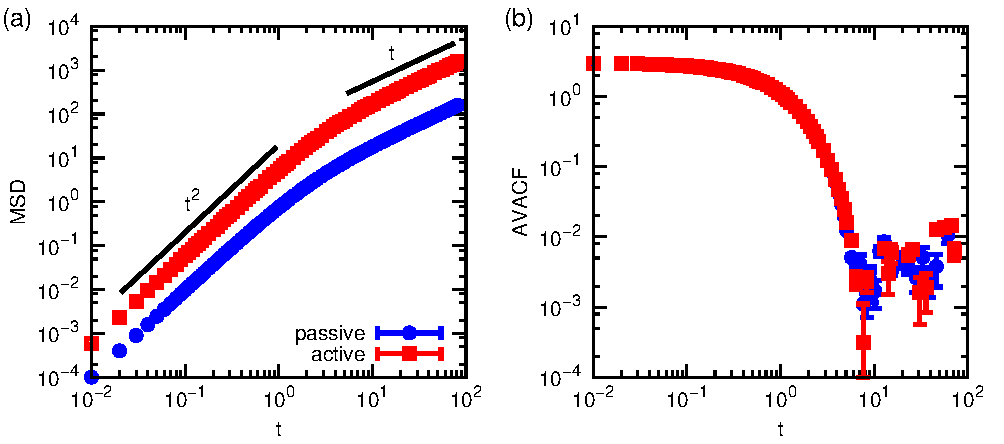
\includegraphics[scale=0.75]{FIGURES/enhanced}
\end{center}
\caption{\label{fig:enhanced}(a) Averaged MSD with standard error for the passive and active particle. The dependence of the MSD on time ($t$) has been indicated with guides to the eye. (b) The AVACF for the same system. Note that the activity does not influence the rotational behavior.}
\end{figure}

Despite the long run length, the quality of the MSD and (A)VACF can be lacking. It is therefore recommended that you output 5 uncorrelated data files. The Python script is designed to facilitate you doing this. Once you have obtained this data for a velocity of \codees{vel=0.0} (passive) and \codees{vel=5.0} active particle, you can average over these and obtain a mean and standard error for your data. You will be pleased to find that indeed, there is enhanced diffusion for the active system and that the ballistic regime is stretched compared to the passive case, see Fig.~\ref{fig:enhanced}(a). Contrasting the passive and active AVACFs shows that the rotational properties are unaffected (Fig.~\ref{fig:enhanced}(b)), as expected.

\section{\label{sec:rectify}Rectification}

In this tutorial you will consider the `rectifying' properties of certain geometries on active systems. Rectification can best be understood by considering a system of passive particles first. In an in-equilibrium system, for which the particles are confined to an asymmetric box, we know that the particle density is homogeneous throughout, provided that there are no external potentials acting on the particles. There are, of course, limitations involving the particle size and the size of the geometry, but for an ideal gas this is certainly true. However, in an out-of-equilibrium setting one can have a heterogeneous distribution of particles, which limits the applicability of an `effective' temperature description. For instance, self-propelled particles will move in a preferred direction a series of wedge-shaped obstacles~\cite{Berdakin13a}. If the obstacles are in a closed tube, then the self-propelled particles will accumulate on one end. Since the speed at which they accumulate depends on their self-motility, different bacteria can be separated in this way~\cite{Berdakin13b}.

\subsection{\label{sub:rgtut}The Rectifying-Geometry Tutorial}

Here, we will set up a rectifying geometry. In the folder EXERCISES you will find the \code{rectification_geometry.py} file. This will help you construct and visualize a rectifying geometry of a cylindrical chamber with a wedge-like obstacle in the center, see Fig.~\ref{fig:system}(a). You will first need to complete the exercises before the script evaluates properly. The wedge-like obstacle causes rectification when the particles are self-propelled. As you can see the LB is used and the rectifying geometry is built up using the \codees{LBBoundary} command, see the User Guide for more information~\cite{UG}. The reason for the use of LB is to help visualize the geometry, as there is currently no means in \es{} or VMD to visualize constraints.

\begin{figure}[!htb]
\begin{center}
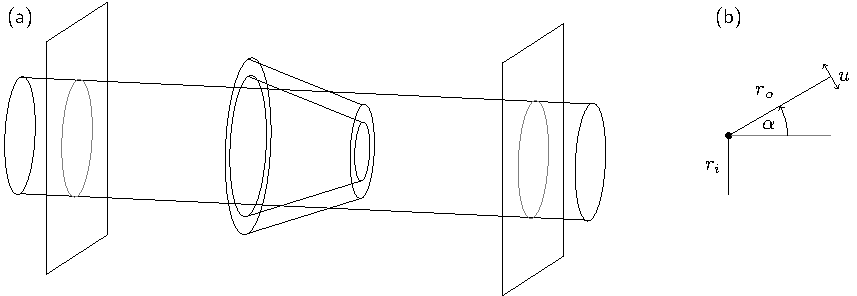
\includegraphics[scale=1.0]{FIGURES/geometry}
\end{center}
\caption{\label{fig:system}(a) Sketch of the rectifying geometry which we simulate for this tutorial. (b) The geometry of the \codees{HollowCone} constraint and \codees{LBBoundary}. The figure is cylindrically symmetric about the x-axis. The size of the pore opening is determined by $r_{i}$, the length of the cone by $r_{o}$ and the opening angle by $\alpha$. Finally, the pore is given a width using the parameter $w$.}
\end{figure}

The first block of the script sets up the basic simulation parameters, with which you should be familiar -- if you are struggling with this part, please consult the previous tutorials. The second block sets up the boundaries using the \codees{LBBoundary} command that was introduced in the LB tutorial. Here it is worth noting that the geometric parameters of the \codees{HollowCone} command are somewhat counterintuitive. They are illustrated in Fig.~\ref{fig:system}(b) for clarification. Finally, in the third block the code
\begin{espresso}
lbf.print_vtk_boundary("{}/boundary.vtk".format(outdir))
\end{espresso}
ensures that the boundary data is exported to a \codees{.vtk} file. This file can be read in and visualized using the program \code{ParaView}, which should have been introduced in the LB and Electrostatics tutorials. Here, we briefly comment on how the geometry can be visualized. In the command prompt type
\begin{bash}
$ paraview &
\end{bash}
to open ParaView. Open the relevant \code{.vtk} file (in our case \code{boundary.vtk}). Click the green \code{Apply} button. Now add a \code{Clip} from the ribbon just above the Pipeline Browser to the highlighted \code{boundary.vtk} entry. Within the \code{Clip} \code{Properties} tab, select \code{Scalar} in the \code{Clip Type} drop-down tab. Then set the value of the scalar to 0.1 with the slide (or by typing in the field) and tick the \code{Inside Out} box. Click \code{Apply}, next slide the \code{Opacity} slide to 0.25, to visualize the inside of the geometry that you have created, see Fig.~\ref{fig:rectify}(a).

\begin{figure}[!htb]
\begin{center}
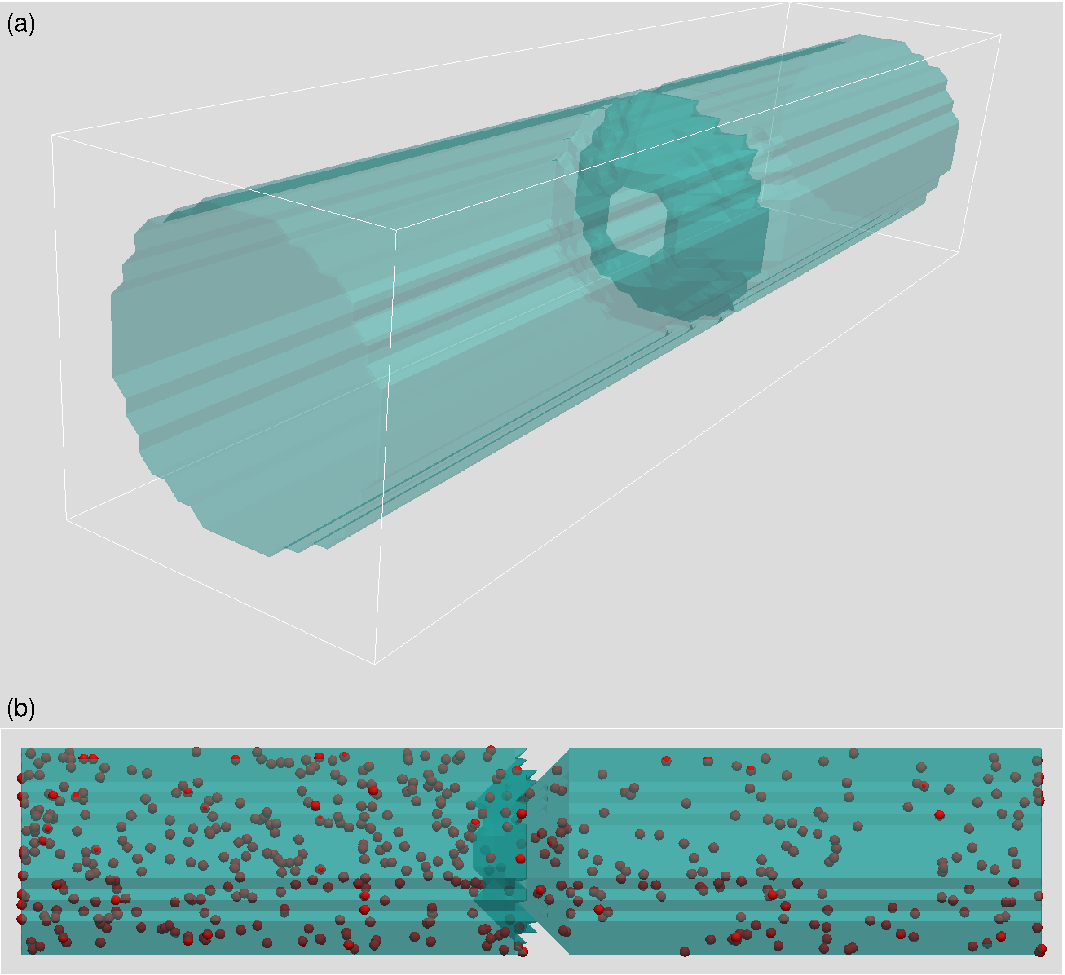
\includegraphics[scale=0.75]{FIGURES/rectify}
\end{center}
\caption{\label{fig:rectify}(a) Snapshot of the rectifying geometry, as visualized with \code{ParaView}. (b) Final state for the system with 500 particles and \codees{vel=5.0}. Note that there are more particles in the left-hand chamber, due to the rectification.}
\end{figure}

\subsection{\label{sub:rstut}The Rectification Tutorial}

Now we will study the effectiveness of our rectifying geometry. In the folder EXERCISES you will find the \code{rectification_simulation.py} file. This Python script will allow the user to appreciate the differences between a passive and an active `ideal gas' in the above geometry. Again, you will have to complete the exercises to obtain a functioning script. N.B. Once up and running, the simulation takes quite a while ($\sim20$ min) on a modern desktop. We recommend that you proceed with the final exercise while the simulation is running.

The first block of the script introduces a procedure to convert a rotation given in spherical coordinates by the azimuthal and polar angle $\theta$ and $\phi$, respectively, to a quaternion. The code
\begin{espresso}
def a2quat(phi,theta):

    q1w = cos(theta/2.0)
    q1x = 0
    q1y = sin(theta/2.0)
    q1z = 0

    q2w = cos(phi/2.0)
    q2x = 0
    q2y = 0
    q2z = sin(phi/2.0)

    q3w = (q1w*q2w-q1x*q2x-q1y*q2y-q1z*q2z)
    q3x = (q1w*q2x+q1x*q2w-q1y*q2z+q1z*q2y)
    q3y = (q1w*q2y+q1x*q2z+q1y*q2w-q1z*q2x)
    q3z = (q1w*q2z-q1x*q2y+q1y*q2x+q1z*q2w)

    return [q3w,q3x,q3y,q3z]
\end{espresso}
essentially implements the geometric relation
\begin{equation}
  \begin{pmatrix}
    w \\ x \\ y \\ z \\
  \end{pmatrix}
  =
  \begin{pmatrix}
    \cos(\alpha/2) \\
    \sin(\alpha/2)\ n_x \\
    \sin(\alpha/2)\ n_y \\
    \sin(\alpha/2)\ n_z \\
  \end{pmatrix}
\end{equation}
where $\alpha$ is the angle and $\mathbf{n} = (n_x,n_y,n_z)$ is the
axis of rotation. This relation is used for both rotation axes and subsequently the two expressions are quaternion multiplied to obtain the full rotation. This procedure will be used later to draw (almost) random quaternions. The rest of the block deals with standard input and output and parameter/simulation definitions.

The second block of the script uses the geometric parameters from the \code{rectification_geometry.py} script to establish the constraints that keep the particles inside of the confining geometry. The relevant \es{} command is \codees{system.constraints.add()} and has already been introduced in the basic tutorial. Next we set up interactions between the geometry and the particles --- in this case the almost-hard WCA interaction --- to ensure that they are trapped. In the fourth block, the geometry is seeded with particles, two clouds of equal size in the respective chambers. This is done to ensure that the equilibration time for the system is limited. That is, if you had set up all particles in a single chamber, there would obviously be flow from the full chamber to the empty one, despite the system being passive (in equilibrium), as the density is homogenized.

\begin{figure}[!htb]
\begin{center}
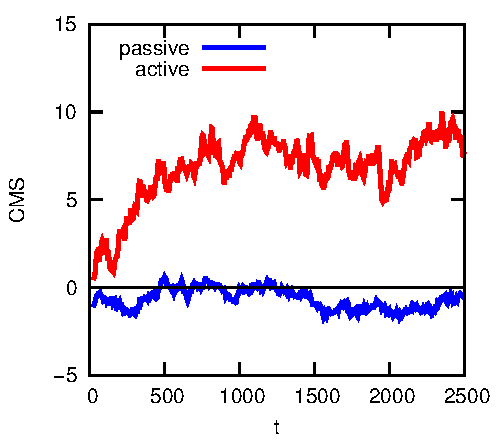
\includegraphics[scale=1.0]{FIGURES/rectification}
\end{center}
\caption{\label{fig:rectification}The change in the position of the CMS for the rectifying geometry with particles. The passive system fluctuates around zero (mid-way in the box), while the active one shows an accumulation of particles in one of the chambers.}
\end{figure}

The final block is concerned with measuring the rectifying properties of this geometry. We do so with a convenient parameter, namely the center of mass (CMS) of the system. You can use the \es{} command \codees{system.galilei.system_CMS()} to determine it directly~\cite{UG}. If the system is passive, then the CMS should fluctuate around the center of the box. However, if there is rectification, this can be seen as a deviation of the CMS from this center. Figure~\ref{fig:rectification} shows the evolution of the CMS as a function of time for passive and active (a velocity of 5.0) particles in the system. The script also outputs a snapshot of the final coordinates of the particles using the line
\begin{espresso}
system.part.writevtk("{}/points_{}.vtk".format(outdir,vel),types=[0])
\end{espresso}
The \codees{writevtk} command outputs the coordinates of the particles of type 0 to a file that is ParaView readable. You can now show how the particles are distributed in the geometry that you visualized in the previous section. To do so, choose the relevant \code{.vtk} file,~\textit{e.g.}, \code{points_5.0.vtk} and load it into ParaView. Now add a \code{Glyph} from the ribbon just above the Pipeline Browser to the highlighted \code{points_5.0.vtk} entry. Select \code{Sphere} from the \code{Glyph Type} drop down. Scroll down and select \code{off} in the \code{Scale Mode} drop down. Tick the \code{Edit} box and set the scale factor to 1.0. As you can see, there are clearly far more particles in the `front' chamber, than there are in the other, see Fig.~\ref{fig:rectify}(b). This can be explained by the fact that the activity makes it easier to take the barrier in one direction than in the other. Or in technical terms: the equivalence between thermodynamic pressure and mechanical pressure is lost.

\section{\label{sec:flow}Flow Field around a Swimmer}

As previously discussed, the flow field around an active particle should not contain a monopolar term. At least, not when there are no other forces acting on the particle. In this tutorial, we will examine the flow field around the two basic types of active swimmer: pushers and pullers. The nature of these flow fields ultimately determine how particles interact with their surroundings. That is, whether they are attracted to walls or repelled by them~\cite{Spagnolie_12}, how they stir tracer beads in the fluid~\cite{Morozov_14}, and how they move collectively~\cite{Zoettl_14}. However, it goes beyond the scope of this tutorial to discuss all of these points in detail.

\subsection{\label{sub:fftut}The Flow-Field Tutorial}

Now we will study the flow field around a simple pusher and puller particle in \es{}. In the folder EXERCISES you will find the \code{flow_field.py} file. Once again, you will have to complete the excercises to obtain a functioning script. The structure of the blocks and their content should by now be straightforward for you to understand on the basis of the previous tutorials and the information provided here. We will therefore focus on the use of this script.

\begin{figure}[!htb]
\begin{center}
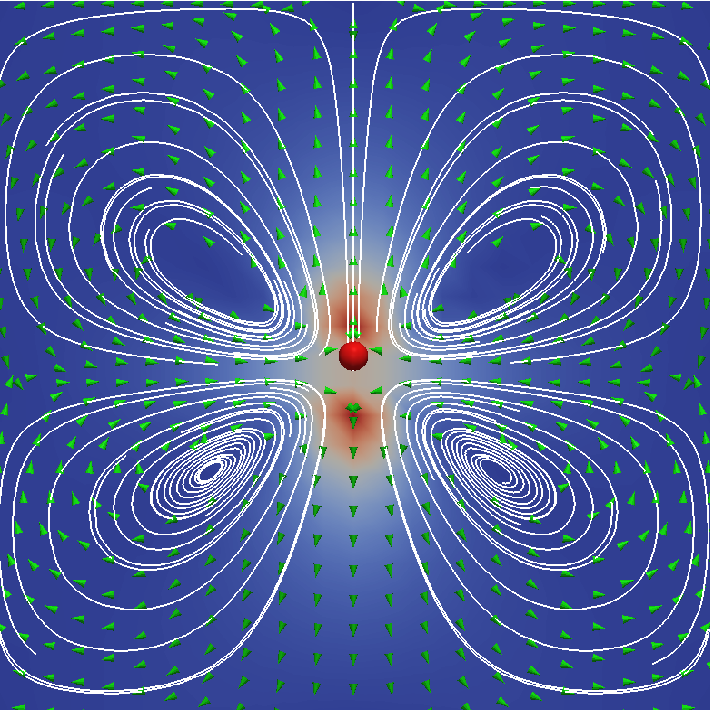
\includegraphics[scale=0.75]{FIGURES/flow_field}
\end{center}
\caption{\label{fig:flow_field}(a) Snapshot of the flow field around a pusher particle visualized with ParaView.}
\end{figure}

First run the simulation for a puller particle and a position of 0.0. This will generate output in the directory that you have set up. Examine the content of this folder and, in particular, the \code{trajectory.dat} file. From the final line of this file, you can determine the position of the swimmer at the end of the run. Now rerun the script with a modified position value, such that the particle ends up in the center of the box. This generates a second directory. Now go into this directory and open ParaView. Using the techniques you have learned in the above tutorial, you can visualize the particle, and using the methods you have picked up in the Electrokinetics tutorial, you can visualize the fluid flow around this particle using,~\textit{e.g.}, stream lines, a slice, or arrows. When you are done, the result could look like Fig.~\ref{fig:flow_field}.

\section{\label{sec:end}Concluding Remarks}

With that, you have come to the end of this tutorial. We hope you found it informative and that you have a sufficient understanding of the way to deal with active matter in \es{} to set up simulations on your own.

\section*{\label{sec:bib}Bibliography}

\bibliographystyle{unsrt}
\bibliography{refs}

\end{document}

%%% Local Variables:
%%% mode: latex
%%% End:
